\item[(a)] Data Generating
Use attached python code to generate the data set.\\
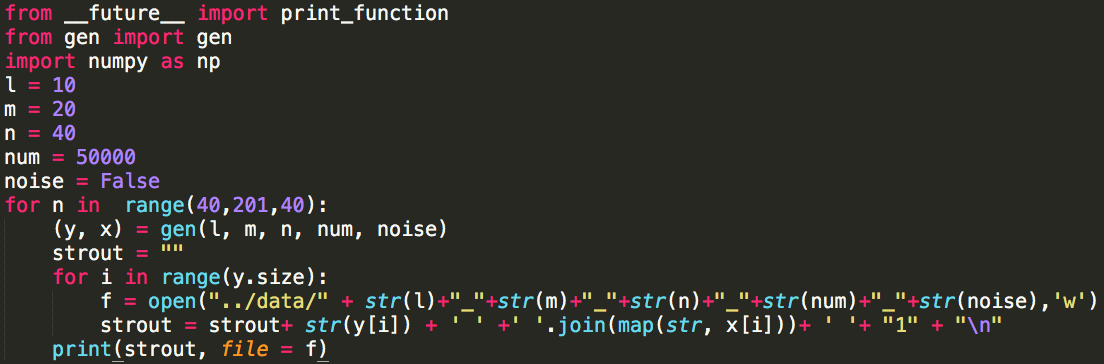
\includegraphics[width = 0.9\textwidth]{pythoncode2.png}

\item[(b)] Parameters Tuning\\
1. For Perceptron, $\eta = 1$, $\gamma = 0$. Nothing needs to be swept.\\ 
2. For Perceptron w/margin, choose $\eta \in \{1.5,0.25,0.03,0.005,0.001\}$, $\gamma = 1$.\\ 
3. For Winnow, choose $\alpha \in \{1.1,1.01,1.005,1.0005,1.0001\}$, $\gamma = 0$.\\
4. For Winnow w/margin, choose $\alpha \in \{1.1,1.01,1.005,1.0005,1.0001\}$, \\$\gamma \in \{2.0,0.3,0.04,0.006,0.001\}$.\\
5. For AdaGrad, choose $\eta \in \{1.5,0.25,0.03,0.005,0.001\}$, $\gamma = 1$.
\end{itemize}
   \begin{center}
    \begin{tabular}{|p{2.2cm}|p{2.5cm}|p{2.5cm}|p{2.5cm}|p{2.5cm}|p{2.5cm}|}
      \hline
      Algorithm  & n=40 & n=80 & n=120& n=160 & n=200\\\hline\hline
      Perceptron &  Accu=0.9998 &   Accu=1&  Accu=0.9994&  Accu=0.9996&  Accu=0.9964\\\hline
      Perceptron w/margin & $\eta$=0.03, Accu=1 & $\eta$=0.03, Accu=1& $\eta$=0.03, Accu=1& $\eta$=0.03, Accu=0.9998& $\eta$=0.03, Accu=0.9974\\\hline
      Winnow   & $\alpha$=1.1, Accu=0.9994 & $\alpha$=1.1, Accu=1& $\alpha$=1.1, Accu=0.9996& $\alpha$=1.1, Accu=1& $\alpha$=1.1, Accu=0.999 \\\hline
      Winnow w/margin   & $\alpha$=1.1, $\gamma=2$, Accu=1 & $\alpha$=1.1, $\gamma=2$, Accu=1& $\alpha$=1.1, $\gamma=2$, Accu=1& $\alpha$=1.1, $\gamma=2$, Accu=1& $\alpha$=1.1, $\gamma=2$, Accu=1 \\\hline
      AdaGrad  & $\eta$=1.5, Accu=1 & $\eta$=1.5, Accu=1& $\eta$=1.5, Accu=1& $\eta$=1.5, Accu=0.9988& $\eta$=1.5, Accu=0.9856 \\\hline
    \end{tabular}
\end{center}

\begin{itemize} 
  \item[(c)] Experiment\\
  Choose the parameters we get above, set the iteration limitation to large enough (I set it to 2000), and start to accumulate the number of mistakes happened until no mistake happen in one iteration. Plot the data x axis means n, order of instance space, and y axis means the number of mistakes made until the algorithm converged.\\
  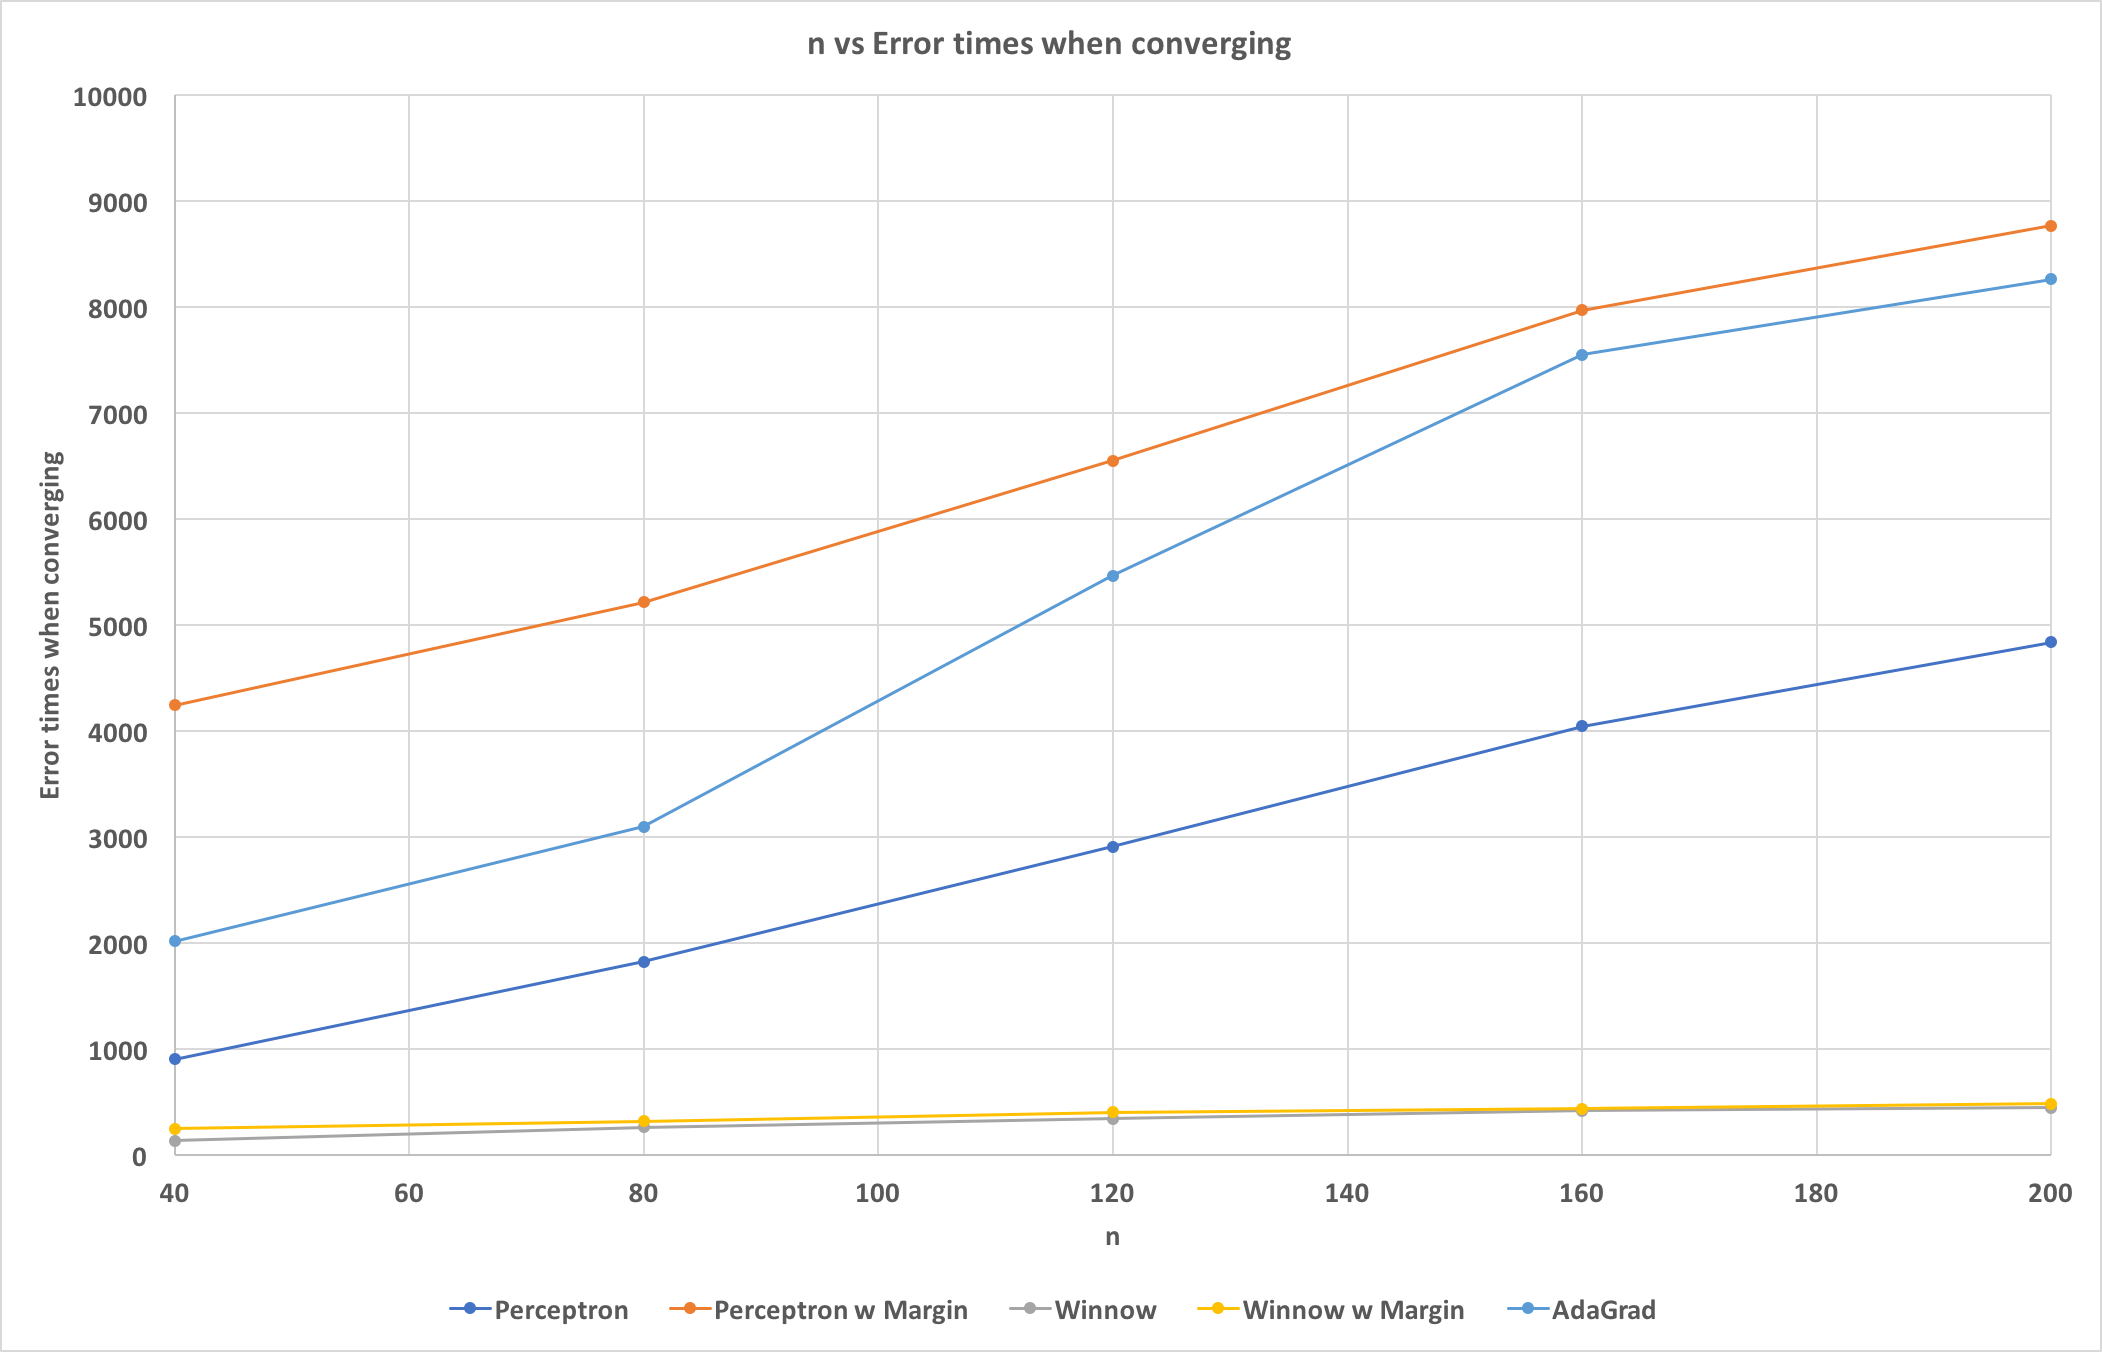
\includegraphics[width = 0.9\textwidth]{n40to200.png}
  To conclude the experiment, the figure shows that: 1. Winnow is the best algorithm in this experiment. 2. Perceptron with margin needs more mistakes to converge. 